% 次に,提案システムが既存システムと比較して異なる特性がある,または課題になる特性が明白である場合,どの程度それらが問題になるのかについて実際に評価すればいい
%評価基準
%Fialure Resilience, Performance(Latency, Misconfiguration, Load Balance)
%サービスとして要求されるもの
% Resolution response time
% Resolution Accuracy
% Resolution guarantee
% Resolution fairness
\section{評価}
\label{sec:evaluation}
提案システムでは,DNSトンネリング抑止の目的に対して,フラットな名前空間とDHTの仕組みを採用している.
このアプローチは,名前解決のパフォーマンスにおいて,コンテンツの識別子に用いられるメッセージダイジェストの算出に伴うメモリ消費と問い合わせノードの探索の処理がオーバーヘッドになることが予想される.
本章では,DNSトンネリング抑止としての提案システム設計の有用性と提案システムの特性について評価した結果を述べる.
%フラットな名前空間とDHTに基づき分散的な管理する提案システムが,DNSトンネリング抑止に対して有効であることを明らかにする.
評価では,提案システムのプロトタイプを実装することで,シミュレーションに基づいて評価を行った.

また,既存システムとの比較に基づいたシミュレーションテストにより,名前解決速度・トラフィック量などの特性を明らかにする.

トンネリング抑止の機能評価テストでは,フルサービスリゾルバとマネージャおよびプロバイダをPython3を用いて実装し,それらサービスをDockerのコンテナとして動作させることによって,提案システムにおける名前解決環境を再現したプロトタイプを用いた.
また,DNSトンネリングの通信には,ランダムなドメイン名をdigコマンドを用いることによって再現した.
プロトタイプ上におけるdigコマンドによる擬似トンネリング通信について,プロバイダにデータが転送されないことを確認する.
特性評価では,ランダムな名前解決クエリを用意し,既存のDNSと提案システムの両方で問い合わせた際のトラフィックと名前解決の速度について,統計的に評価を実施する.

表~\cite{tab:diff_feature}で示す通り,既存システムと提案システムでは以下のような特性の違いがある.
本節では,これら特性の違いを踏まえて,DNS-TDにおける名前解決のパフォーマンスとトラフィック量に明らかにする.
\begin{table}[htb]
 \caption{DNSとDNS-TDの特性比較}
 \centering
  \begin{tabular}{lll}
    \toprule
		 & \multicolumn{1}{c}{\textbf{DNS}} & \multicolumn{1}{c}{\textbf{DNS-TD}} \\
    \midrule
    \ \textbf{ドメイン長} & \begin{tabular}{l}変長\\(最大253byte)\end{tabular} & \begin{tabular}{l}固定長(72byte)\\(コンテンツID(56) \& \\ ドメインID(16))\end{tabular} \\ \hline
    \textbf{\begin{tabular}{l}トランザクション\\試行回数\end{tabular}} &\ ラベルに依存 & 1 \\ \hline
    \ \textbf{RTT} & \begin{tabular}{l}全ての権威サーバ\\とのRTT総和\end{tabular} & マネージャとのRTTのみ  \\ \hline
		\ \textbf{ゾーンファイル} &\ ファイル & インメモリデータベース\\ \hline
		\ \textbf{その他} & & \begin{tabular}{l}・ハッシュ計算の発生\\・マネージャ探索\end{tabular}\\
    \bottomrule
  \end{tabular}
 \label{tab:diff_feature}
\end{table}


\subsection{プロトタイプ実装}
検証環境には,Dockerを使用し,コンテナ同士の接続によってDNSのチェーンを実現する.
その概略図は,以下の通りである.

\subsection{名前解決機能のシュミレーションテスト}
\label{sec:eval-tunnel}
提案システムDNS-TDにおける名前解決の動作を明らかにするために,本項では実際にシステムをDocker環境上で動作させたシミュレーションの結果を説明する.
提案システムのDNS Exfiltrationへの機能性について評価した結果を述べる.

%実際にコンテンツが登録されている場合とコンテンツ情報が含まれていない場合(DNSクエリ)
%擬似DNSトンネリングとするドメイン名については,過去の文字列分布が均等分布になることに基づいてランダムな関数で作成したこと理論について説明すること
%提案システム上で,iodineを動作させた際のパケットキャプチャーした様子を説明する

\begin{figure}[p]
 \centering
 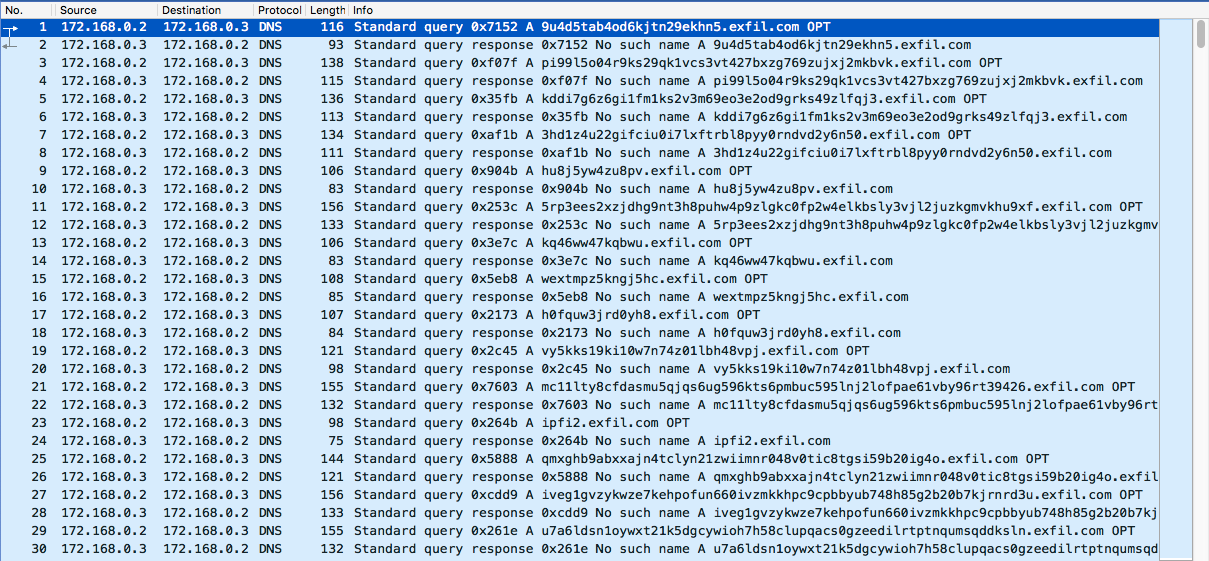
\includegraphics[width=14.5cm]{figure/stab-fullservice.png}
 \vspace{-1cm}
 \caption{スタブリゾルバからフルサービスリゾルバにおける通信}
 \label{fig:fullservice-manager}
 \vspace{1cm}
 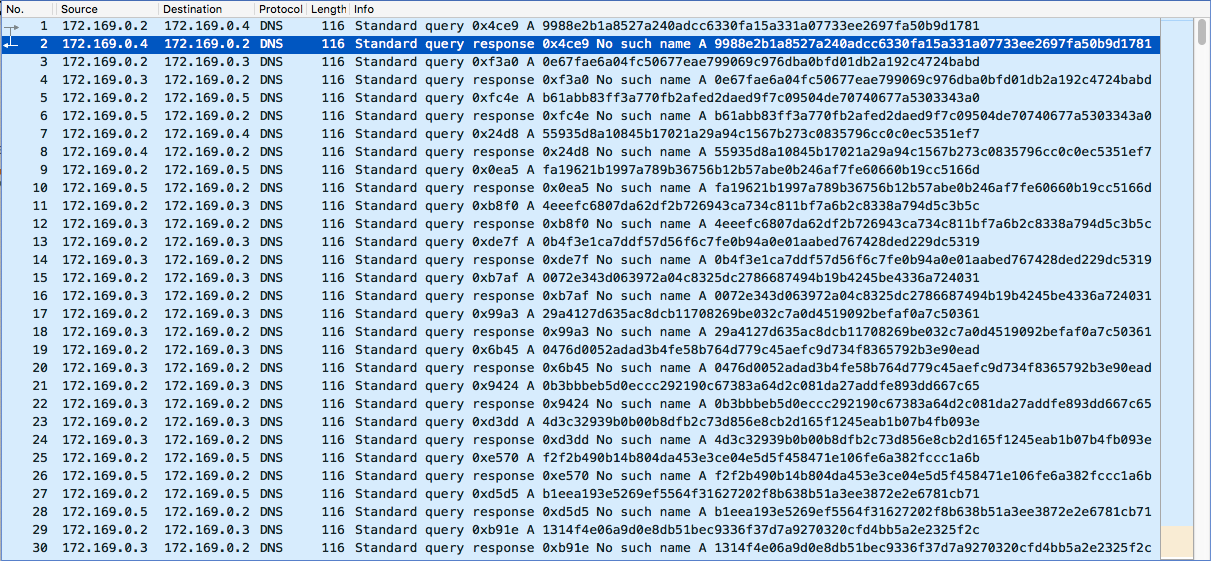
\includegraphics[width=14.5cm]{figure/fullresolver-manager.png}
 \vspace{-1cm}
 \caption{フルサービスリゾルバからマネージャにおける通信}
 \label{fig:fullservice-manager}
\end{figure}

\newpage
\subsection{要素別}
\subsubsection{トラフィック量}
%クエリminimizationがどの程度普及しているのかによって,計算方法が随分と異なることが予想される
%Query minimizationの場合は,どのようになるのか
第~\ref{sec:resolution_speed}項で述べるように,DNSではサーバに再帰的に問い合わせることで名前が解決されるのに対して,DNS-TDではサーバへの問い合わせは一度で済む.
このため,DNS-TDでは,DNSと比べて少ないトラフィック頻度となることが予想される.
しかし,パケットサイズに関して,DNSではドメイン名から
他方で,DNS-TDでは固定長のドメイン名がサーバに問い合わせられるのに対して,

DNSでは,ゾーンをドメインごとに分割し,フルサービスリゾルバはルート権威サーバから目的の権威サーバに向かって再帰的に問い合わせ,権威サーバのアドレスを解決しながら,最終的にコンテンツを保持する権威サーバからコンテンツを取得する.

\begin{figure}[h]
 \centering
 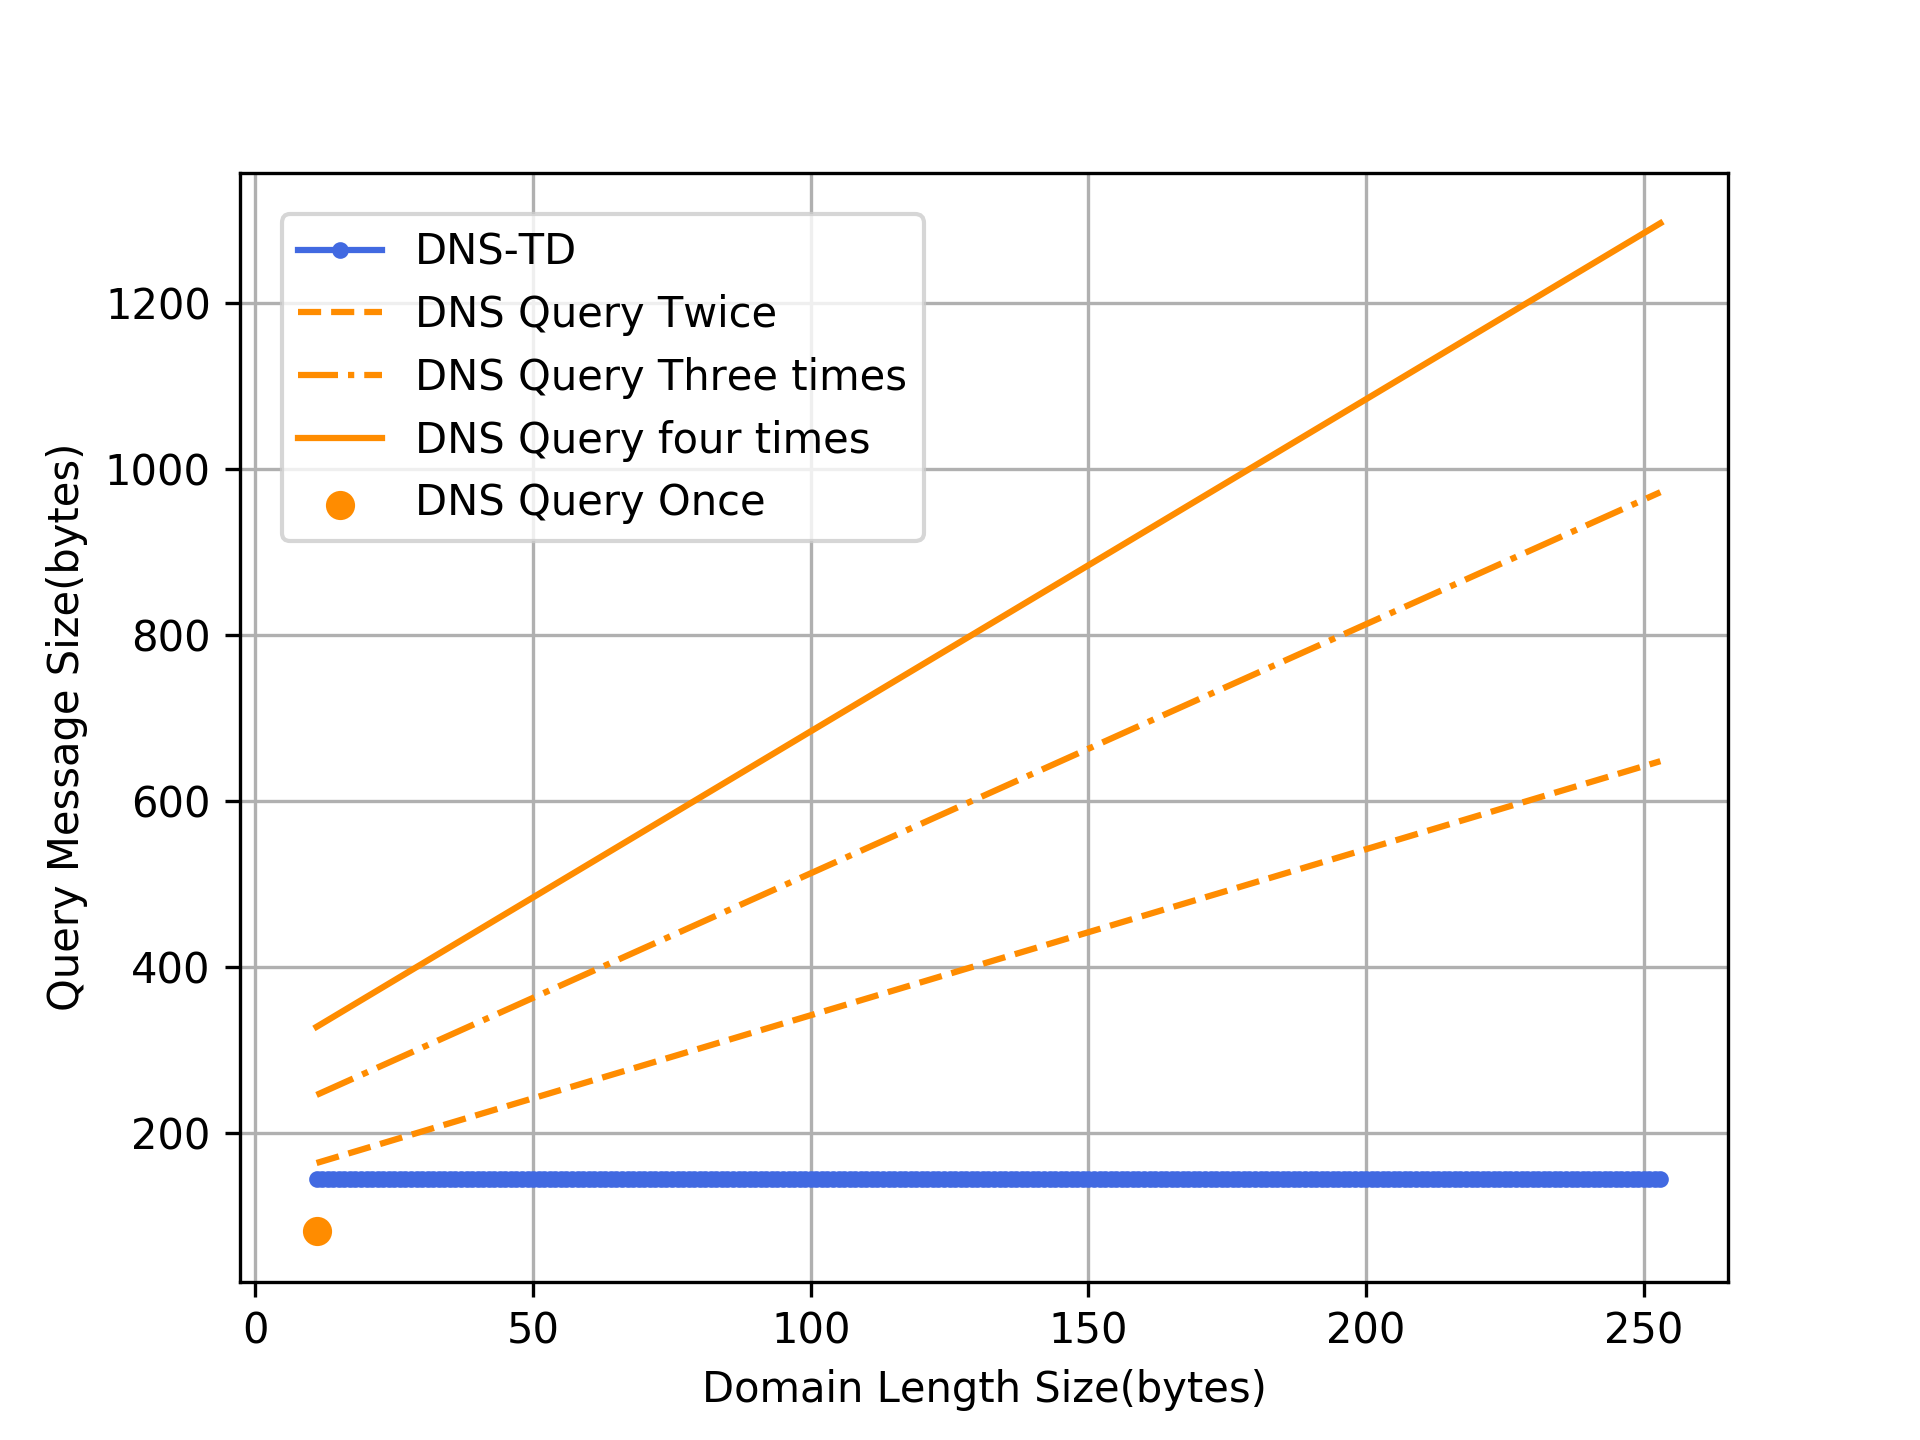
\includegraphics[scale=0.8]{figure/length-size.png}
 \caption{DNS-TDとDNSにおける名前解決に使用されるクエリパケットサイズの比較}
 \label{fig:length-size}
\end{figure}

本項では,提案手法におけるトラフィックについて評価する.
DNS-TDでは,シンボル志向の名前解決メソッドによって,既存の再帰問い合わせによるメソッドよりも少ないトラフィックに抑えることが期待される.
DNS-TDでは,クエリ数とトラフィック量は比例関係にある.
他方で,新たにマネージャ間通信という従来にはないトラフィックが発生する.
本項では,これトラフィックがネットワーク全体にどの程度影響を及ぼすのかについて評価する.

\newpage
\subsubsection{オーバヘッド}
%ハッシュ計算に伴うオーバーヘッドについて
提案システムの名前解決において,フルサービスリゾルバは,コンテンツIDの値を算出して初めてマネージャノードを特定することができる仕様になっている.
また,コンテンツIDの重複を防止するための仕様には,ドメイン名から算出されるドメインIDが使用される.
以上のことから,提案システムのフルサービスリゾルバは,名前解決にあたって2回のハッシュ値の計算処理を行う必要がある.
これは,既存システムにはない処理工程のため,既存システムとのパフォーマンスを評価する際にオーバーヘッドになると予想される.
本項では,既存システムにはないこのハッシュ値の計算処理について,5000回のハッシュ値の計算実験に基づいて評価する.

評価には,

問い合わせられたドメイン名とレコードタイプからコンテンツIDおよびドメインIDを算出し,
にどのよかについて,名前解決にかかる平均時間によって評価する.
本項では,提案システムにおける名前解決処理のオーバーヘッドとして懸念されるハッシュ値計算処理について,評価した結果を示す.
提案システムの名前解決処理において,フルサービスリゾルバはスタブリゾルバからのクエリを問い合わせる宛先ノードをクエリされたドメイン名とクエリタイプからハッシュ値を算出することで決定される.
既存システムのように``Root.hints''ファイルを用いて,
フルサービスリゾルバは最初の転送先となるルート権威サーバのアドレスが確認できるは保持していない.

マネージャノードは,スタブリゾルバから問い合わせられたドメイン名とレコードタイプから算出されるコンテンツIDに基づいて決まる.
このため,フルサービスリゾルバは,スタブリゾルバからのクエリをサーバに転送する処理に加えて,コンテンツIDの算出処理を実行する必要がある.
コンテンツIDは,ドメイン名とレコードタイプの和をメッセージとするハッシュ関数から算出されるメッセージダイジェストである.
以上のことから,DNS-TDでは,コンテンツIDの算出に伴う処理が名前解決におけるパフォーマンスのオーバーヘッドになることが予想される.
%処理にかかるメモリおよび時間のオーバーヘッドについて調べた.

\begin{figure}[h]
 \centering
 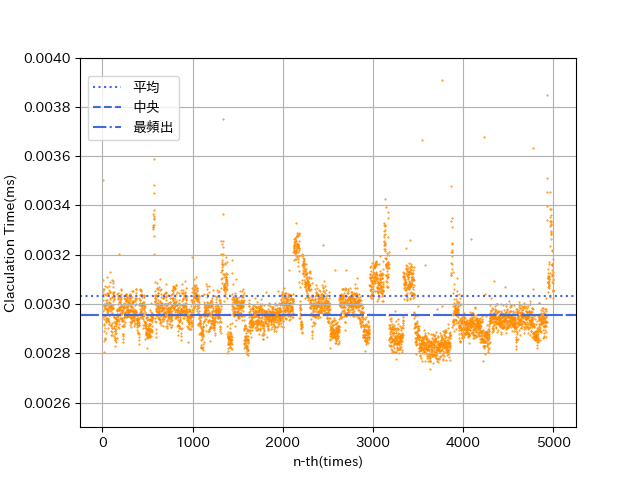
\includegraphics[scale=0.8]{figure/overhead.png}
 \caption{コンテンツIDとドメインID算出にかかる計算時間のオーバーヘッド}
 \label{fig:overhead}
\end{figure}

DNS-TDで使用されるハッシュ関数には,224bitの名前空間をもつsha3というハッシュ関数が用いられている.
%DNSは,現在のインターネットの根幹に位置する技術であるため,DNSトラフィックはインターネット全体に大きく影響する.
\newpage
\subsubsection{名前解決速度}
\label{sec:resolution_speed}
DNS-TDにおけるゾーンは,ソートされたハッシュ名前空間の範囲によって分割されているため,コンテンツIDから担当のコンテンツサーバを一意に求めることができる.
他方で,既存システムのDNSでは,ドメイン名の階層構造と委譲の仕組み基づいてゾーンが分割されているため,コンテンツを保持する権威サーバにはルート権威サーバから再帰的に問い合わせる必要がある.
このため,既存システムでは,ドメイン名においてドメインが委譲された分だけ権威サーバに問い合わせる必要がある.
以上のように,DNS-TDとDNSの名前解決処理には,サーバに問い合わせる数の違いがある.
そこで,本項では,サーバへの問い合わせ数の違いが名前解決の速度にどの程度影響を及ぼすのかについて調べた.

本項では,DNS-TDが識別子から一意にレコード情報にアクセス可能である点について,DNSとの比較評価を行う.
DNS-TDの名前解決では,
従来のDNSでは,ラベルごとにゾーンが移譲されている場合,レコード情報を保持するノードまでのホップ数はラベル数nに比例する.
それに対して,DNS-TDでは,識別子から一意にレコード情報を保持するマネージャノードを特定できるので,常にホップ数は2である.
このため,既存の名前解決システムより速度の向上が期待される.
% 既存のDNSにおけるラウンドトリップのうち,再帰問い合わせの最後の権威サーバRTTがdns-tdのフルリゾルバとマネージャのそれになる.
% 遠いものと近いもののRTTを用意する必要がある
% 実装する必要はない.理論で評価できる
% あえてするとすれば,フルサービスリゾルバとマネージャ間通信
% DDoSへの影響については,リクエストとレスポンスパケットのサイズからアンプ率に着目する
DNS-TDでは,56byteを固定長とするコンテンツIDをシンボルとすることによって,レコード情報にアクセスする.
この仕組みの影響で,DNS-TDのパケットは従来のパケットと比較して肥大する特性がある.
このため,送信元を目的ホストと偽装することで目的ホストの計算リソースを圧迫するDDoS攻撃に対して,脅威を高める可能性が予想される.

\begin{figure}[h]
 \centering
 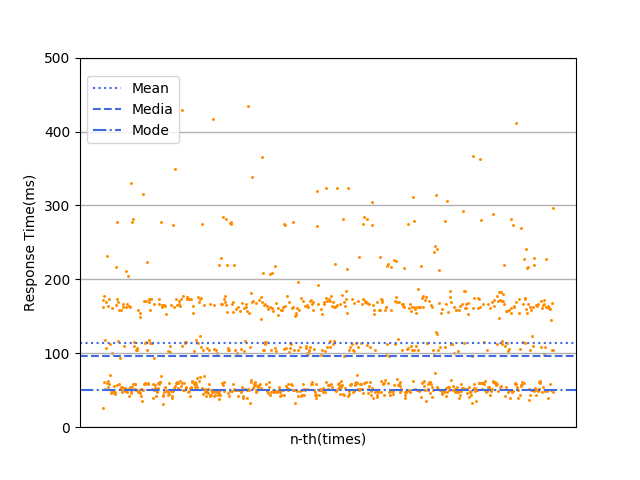
\includegraphics[scale=0.8]{figure/root-rtt.png}
 \caption{Root権威サーバにおけるRTTの分布}
 \label{fig:root-rtt}
\end{figure}

\begin{figure}[h]
 \centering
 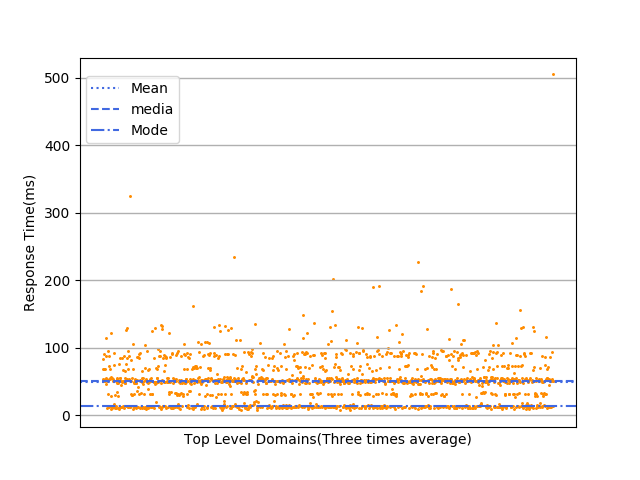
\includegraphics[scale=0.8]{figure/average_rtt.png}
 \caption{TLD権威サーバにおけるRTTの分布}
 \label{fig:tlr-rtt}
\end{figure}

% 比較項目
% * 平均したドメイン長と
% マネージャが攻撃された場合の影響は,世界規模に影響する.
% 従来のドメインごとにゾーンが分離している設計と違い,一つのゾーンには様々な組織のドメインが管理されている.
% このゾーンを全て書き換えることができることは脅威である.
% アンプ率は,既存のDNSと基本的に変わらない.DNSSECがあるかないかについて議論するくらい
%既存システムにおけるドメイン長の平均
